% Options for packages loaded elsewhere
\PassOptionsToPackage{unicode}{hyperref}
\PassOptionsToPackage{hyphens}{url}
%
\documentclass[
  ignorenonframetext,
  aspectratio=169,
  chinese-hans,
]{beamer}
\usepackage{pgfpages}
\setbeamertemplate{caption}[numbered]
\setbeamertemplate{caption label separator}{: }
\setbeamercolor{caption name}{fg=normal text.fg}
\beamertemplatenavigationsymbolshorizontal
% Prevent slide breaks in the middle of a paragraph
\widowpenalties 1 10000
\raggedbottom
\setbeamertemplate{part page}{
  \centering
  \begin{beamercolorbox}[sep=16pt,center]{part title}
    \usebeamerfont{part title}\insertpart\par
  \end{beamercolorbox}
}
\setbeamertemplate{section page}{
  \centering
  \begin{beamercolorbox}[sep=12pt,center]{section title}
    \usebeamerfont{section title}\insertsection\par
  \end{beamercolorbox}
}
\setbeamertemplate{subsection page}{
  \centering
  \begin{beamercolorbox}[sep=8pt,center]{subsection title}
    \usebeamerfont{subsection title}\insertsubsection\par
  \end{beamercolorbox}
}
\AtBeginPart{
  \frame{\partpage}
}
\AtBeginSection{
  \ifbibliography
  \else
    \frame{\sectionpage}
  \fi
}
\AtBeginSubsection{
  \frame{\subsectionpage}
}

\usepackage{amsmath,amssymb}
\usepackage{iftex}
\ifPDFTeX
  \usepackage[T1]{fontenc}
  \usepackage[utf8]{inputenc}
  \usepackage{textcomp} % provide euro and other symbols
\else % if luatex or xetex
  \usepackage{unicode-math}
  \defaultfontfeatures{Scale=MatchLowercase}
  \defaultfontfeatures[\rmfamily]{Ligatures=TeX,Scale=1}
\fi
\usepackage{lmodern}
\usetheme[]{Copenhagen}
\usecolortheme{default}
\usefonttheme{serif}
\ifPDFTeX\else  
    % xetex/luatex font selection
\fi
% Use upquote if available, for straight quotes in verbatim environments
\IfFileExists{upquote.sty}{\usepackage{upquote}}{}
\IfFileExists{microtype.sty}{% use microtype if available
  \usepackage[]{microtype}
  \UseMicrotypeSet[protrusion]{basicmath} % disable protrusion for tt fonts
}{}
\makeatletter
\@ifundefined{KOMAClassName}{% if non-KOMA class
  \IfFileExists{parskip.sty}{%
    \usepackage{parskip}
  }{% else
    \setlength{\parindent}{0pt}
    \setlength{\parskip}{6pt plus 2pt minus 1pt}}
}{% if KOMA class
  \KOMAoptions{parskip=half}}
\makeatother
\usepackage{xcolor}
\newif\ifbibliography
\setlength{\emergencystretch}{3em} % prevent overfull lines
\setcounter{secnumdepth}{-\maxdimen} % remove section numbering


\providecommand{\tightlist}{%
  \setlength{\itemsep}{0pt}\setlength{\parskip}{0pt}}\usepackage{longtable,booktabs,array}
\usepackage{calc} % for calculating minipage widths
\usepackage{caption}
% Make caption package work with longtable
\makeatletter
\def\fnum@table{\tablename~\thetable}
\makeatother
\usepackage{graphicx}
\makeatletter
\newsavebox\pandoc@box
\newcommand*\pandocbounded[1]{% scales image to fit in text height/width
  \sbox\pandoc@box{#1}%
  \Gscale@div\@tempa{\textheight}{\dimexpr\ht\pandoc@box+\dp\pandoc@box\relax}%
  \Gscale@div\@tempb{\linewidth}{\wd\pandoc@box}%
  \ifdim\@tempb\p@<\@tempa\p@\let\@tempa\@tempb\fi% select the smaller of both
  \ifdim\@tempa\p@<\p@\scalebox{\@tempa}{\usebox\pandoc@box}%
  \else\usebox{\pandoc@box}%
  \fi%
}
% Set default figure placement to htbp
\def\fps@figure{htbp}
\makeatother

\usepackage{ctex}
\usepackage{graphicx}
\makeatletter
\@ifpackageloaded{caption}{}{\usepackage{caption}}
\AtBeginDocument{%
\ifdefined\contentsname
  \renewcommand*\contentsname{目录}
\else
  \newcommand\contentsname{目录}
\fi
\ifdefined\listfigurename
  \renewcommand*\listfigurename{图索引}
\else
  \newcommand\listfigurename{图索引}
\fi
\ifdefined\listtablename
  \renewcommand*\listtablename{表索引}
\else
  \newcommand\listtablename{表索引}
\fi
\ifdefined\figurename
  \renewcommand*\figurename{图}
\else
  \newcommand\figurename{图}
\fi
\ifdefined\tablename
  \renewcommand*\tablename{表}
\else
  \newcommand\tablename{表}
\fi
}
\@ifpackageloaded{float}{}{\usepackage{float}}
\floatstyle{ruled}
\@ifundefined{c@chapter}{\newfloat{codelisting}{h}{lop}}{\newfloat{codelisting}{h}{lop}[chapter]}
\floatname{codelisting}{列表}
\newcommand*\listoflistings{\listof{codelisting}{列表索引}}
\makeatother
\makeatletter
\makeatother
\makeatletter
\@ifpackageloaded{caption}{}{\usepackage{caption}}
\@ifpackageloaded{subcaption}{}{\usepackage{subcaption}}
\makeatother

\ifLuaTeX
\usepackage[bidi=basic]{babel}
\else
\usepackage[bidi=default]{babel}
\fi
\babelprovide[main,import]{chinese-hans}
% get rid of language-specific shorthands (see #6817):
\let\LanguageShortHands\languageshorthands
\def\languageshorthands#1{}
\usepackage{bookmark}

\IfFileExists{xurl.sty}{\usepackage{xurl}}{} % add URL line breaks if available
\urlstyle{same} % disable monospaced font for URLs
\hypersetup{
  pdftitle={监督学习(下)},
  pdfauthor={汪小圈},
  pdflang={zh-Hans},
  hidelinks,
  pdfcreator={LaTeX via pandoc}}


\title{监督学习(下)}
\author{汪小圈}
\date{2025-03-17}

\begin{document}
\frame{\titlepage}


\begin{frame}{内容安排}
\phantomsection\label{ux5185ux5bb9ux5b89ux6392}
\begin{itemize}
\tightlist
\item
  神经网络基础

  \begin{itemize}
  \tightlist
  \item
    浅层神经网络 (Shallow Neural Networks)
  \item
    深层神经网络 (Deep Neural Networks)
  \item
    损失函数 (Loss Functions)
  \item
    模型拟合 (Model Fitting)
  \item
    梯度下降与优化 (Gradients \& Optimization)
  \item
    参数初始化 (Initialization)
  \item
    性能评估 (Performance)
  \item
    正则化方法 (Regularization)
  \end{itemize}
\item
  深度学习简介

  \begin{itemize}
  \tightlist
  \item
    深度学习基本概念
  \item
    常见深度学习架构
  \end{itemize}
\end{itemize}
\end{frame}

\begin{frame}{回顾:集成学习的核心思想}
\phantomsection\label{ux56deux987eux96c6ux6210ux5b66ux4e60ux7684ux6838ux5fc3ux601dux60f3}
\begin{itemize}
\item
  \textbf{集成学习}是一种将\textbf{多个弱学习器 (Weak Learner)
  组合成一个强学习器 (Strong Learner) 的技术}
\item
  \textbf{核心思想:``三个臭皮匠,顶个诸葛亮''}

  \begin{itemize}
  \tightlist
  \item
    组合多个弱学习器的预测结果,获得更全面、更鲁棒的预测能力
  \end{itemize}
\item
  \textbf{降低误差的方式}:

  \begin{itemize}
  \tightlist
  \item
    \textbf{降低方差}:通过并行训练多个基学习器,对结果平均或投票(如Bagging)
  \item
    \textbf{降低偏差}:通过串行训练基学习器,每个学习器纠正前一个的错误(如Boosting)
  \item
    \textbf{提高鲁棒性}:对异常值和噪声数据具有更强的抵抗力
  \end{itemize}
\end{itemize}
\end{frame}

\begin{frame}{回顾:集成学习主要方法}
\phantomsection\label{ux56deux987eux96c6ux6210ux5b66ux4e60ux4e3bux8981ux65b9ux6cd5}
\begin{itemize}
\tightlist
\item
  \textbf{Bagging (Bootstrap Aggregating)}

  \begin{itemize}
  \tightlist
  \item
    并行集成,通过自助采样创建多个训练数据集
  \item
    典型代表:随机森林
  \end{itemize}
\item
  \textbf{Boosting (提升法)}

  \begin{itemize}
  \tightlist
  \item
    串行集成,每个新的基学习器都试图纠正前一个的错误
  \item
    典型代表:AdaBoost、GBDT
  \end{itemize}
\item
  \textbf{Stacking (堆叠法)}

  \begin{itemize}
  \tightlist
  \item
    层次集成,使用另一个学习器组合基学习器的输出
  \item
    在各种机器学习竞赛中广泛应用
  \end{itemize}
\end{itemize}
\end{frame}

\begin{frame}{神经网络简介 (Neural Network)}
\phantomsection\label{ux795eux7ecfux7f51ux7edcux7b80ux4ecb-neural-network}
\begin{itemize}
\item
  \textbf{神经网络}是一种模拟生物神经系统的\textbf{计算模型}
\item
  \textbf{基本结构}:

  \begin{itemize}
  \tightlist
  \item
    由大量相互连接的神经元组成
  \item
    能学习复杂的非线性关系
  \item
    具有强大的模式识别能力
  \end{itemize}
\item
  \textbf{历史发展}:

  \begin{itemize}
  \tightlist
  \item
    1943年:McCulloch和Pitts提出第一个神经元模型
  \item
    1958年:Rosenblatt提出感知机
  \item
    1986年:反向传播算法提出
  \item
    2006年:深度学习兴起
  \item
    2012年:AlexNet赢得ImageNet挑战赛,标志深度学习的突破
  \end{itemize}
\end{itemize}

\begin{figure}[H]

{\centering \includegraphics[width=0.7\linewidth,height=\textheight,keepaspectratio]{images/nn_history.png}

}

\caption{神经网络发展历程}

\end{figure}%
\end{frame}

\begin{frame}{1. 浅层神经网络 - 感知机模型}
\phantomsection\label{ux6d45ux5c42ux795eux7ecfux7f51ux7edc---ux611fux77e5ux673aux6a21ux578b}
\begin{itemize}
\item
  \textbf{感知机 (Perceptron)} 是最基本的神经元模型
\item
  \textbf{单个神经元组成}:

  \begin{itemize}
  \tightlist
  \item
    \textbf{输入 (x₁, x₂, \ldots, xₙ)}:特征向量
  \item
    \textbf{权重 (w₁, w₂, \ldots, wₙ)}:特征重要性
  \item
    \textbf{偏置 (b)}:调整激活阈值
  \item
    \textbf{加权求和}:\(z = \sum_{i=1}^{n} w_i x_i + b\)
  \item
    \textbf{激活函数}:\(a = \sigma(z)\)
  \item
    \textbf{输出}:\(\hat{y} = a\)
  \end{itemize}
\end{itemize}

\begin{figure}[H]

{\centering 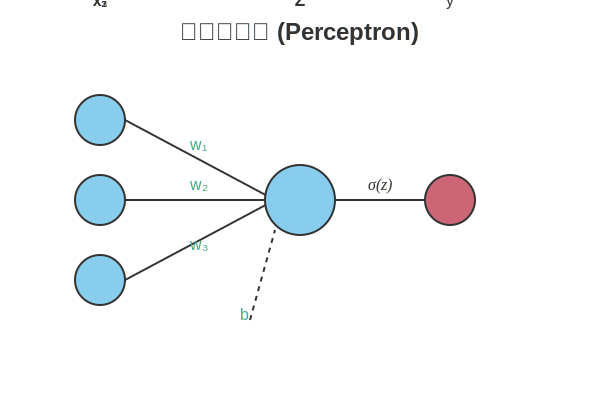
\includegraphics[width=0.6\linewidth,height=\textheight,keepaspectratio]{images/perceptron.png}

}

\caption{感知机模型}

\end{figure}%
\end{frame}

\begin{frame}{1. 浅层神经网络 - 单层感知机局限性}
\phantomsection\label{ux6d45ux5c42ux795eux7ecfux7f51ux7edc---ux5355ux5c42ux611fux77e5ux673aux5c40ux9650ux6027}
\begin{itemize}
\tightlist
\item
  \textbf{线性可分性限制}:

  \begin{itemize}
  \tightlist
  \item
    单层感知机只能解决线性可分问题
  \item
    无法解决XOR等非线性问题
  \end{itemize}
\end{itemize}

\begin{figure}[H]

{\centering 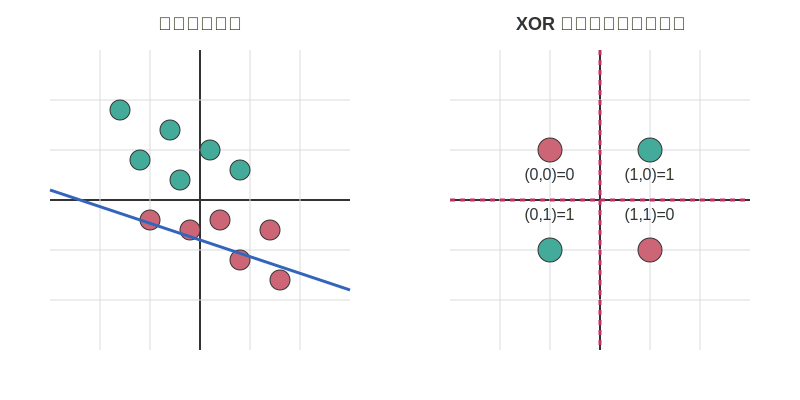
\includegraphics[width=0.7\linewidth,height=\textheight,keepaspectratio]{images/linear_separable.png}

}

\caption{线性可分与非线性可分问题}

\end{figure}%

\begin{itemize}
\tightlist
\item
  \textbf{解决方案}:

  \begin{itemize}
  \tightlist
  \item
    引入多层结构
  \item
    使用非线性激活函数
  \end{itemize}
\end{itemize}
\end{frame}

\begin{frame}{1. 浅层神经网络 - 激活函数}
\phantomsection\label{ux6d45ux5c42ux795eux7ecfux7f51ux7edc---ux6fc0ux6d3bux51fdux6570}
\begin{itemize}
\item
  \textbf{激活函数}引入非线性,是神经网络强大表达能力的关键
\item
  \textbf{常用激活函数}:

  \begin{itemize}
  \tightlist
  \item
    \textbf{Sigmoid}:\(\sigma(z) = \frac{1}{1 + e^{-z}}\)

    \begin{itemize}
    \tightlist
    \item
      输出范围(0,1),适合二分类
    \item
      缺点:存在梯度消失问题
    \end{itemize}
  \item
    \textbf{Tanh}:\(\tanh(z) = \frac{e^z - e^{-z}}{e^z + e^{-z}}\)

    \begin{itemize}
    \tightlist
    \item
      输出范围(-1,1),零中心化
    \item
      仍存在梯度消失问题
    \end{itemize}
  \item
    \textbf{ReLU}:\(\text{ReLU}(z) = \max(0, z)\)

    \begin{itemize}
    \tightlist
    \item
      计算简单,缓解梯度消失
    \item
      可能出现''神经元死亡''问题
    \end{itemize}
  \end{itemize}
\end{itemize}

\begin{figure}[H]

{\centering \includegraphics[width=0.7\linewidth,height=\textheight,keepaspectratio]{images/activation_functions.png}

}

\caption{常见激活函数}

\end{figure}%
\end{frame}

\begin{frame}{1. 浅层神经网络 - 多层感知机}
\phantomsection\label{ux6d45ux5c42ux795eux7ecfux7f51ux7edc---ux591aux5c42ux611fux77e5ux673a}
\begin{itemize}
\item
  \textbf{多层感知机 (MLP)} 是浅层神经网络的典型代表
\item
  \textbf{基本结构}:

  \begin{itemize}
  \tightlist
  \item
    \textbf{输入层}:接收原始特征
  \item
    \textbf{隐藏层}:通常1-2层,提取特征
  \item
    \textbf{输出层}:产生预测结果
  \end{itemize}
\item
  \textbf{前向传播}:信息从输入层流向输出层

  \begin{itemize}
  \tightlist
  \item
    \(\mathbf{z}^{[1]} = \mathbf{W}^{[1]} \mathbf{x} + \mathbf{b}^{[1]}\)
  \item
    \(\mathbf{a}^{[1]} = \sigma(\mathbf{z}^{[1]})\)
  \item
    \(\mathbf{z}^{[2]} = \mathbf{W}^{[2]} \mathbf{a}^{[1]} + \mathbf{b}^{[2]}\)
  \item
    \(\mathbf{a}^{[2]} = \sigma(\mathbf{z}^{[2]})\)
  \end{itemize}
\end{itemize}

\begin{figure}[H]

{\centering \includegraphics[width=0.6\linewidth,height=\textheight,keepaspectratio]{images/mlp.png}

}

\caption{多层感知机结构}

\end{figure}%
\end{frame}

\begin{frame}{2. 深层神经网络 - 基本概念}
\phantomsection\label{ux6df1ux5c42ux795eux7ecfux7f51ux7edc---ux57faux672cux6982ux5ff5}
\begin{itemize}
\item
  \textbf{深层神经网络} 包含多个隐藏层(通常\textgreater2层)
\item
  \textbf{深度学习优势}:

  \begin{itemize}
  \tightlist
  \item
    \textbf{层次化特征学习}:低层学习简单特征,高层学习复杂特征
  \item
    \textbf{表达能力增强}:可以拟合更复杂的函数
  \item
    \textbf{参数效率}:相比宽而浅的网络,参数利用更高效
  \end{itemize}
\item
  \textbf{挑战}:

  \begin{itemize}
  \tightlist
  \item
    训练困难(梯度消失/爆炸)
  \item
    需要大量数据
  \item
    计算资源需求高
  \item
    过拟合风险增加
  \end{itemize}
\end{itemize}

\begin{figure}[H]

{\centering \includegraphics[width=0.65\linewidth,height=\textheight,keepaspectratio]{images/deep_nn_features.png}

}

\caption{深层神经网络与特征层次}

\end{figure}%
\end{frame}

\begin{frame}{2. 深层神经网络 - 表达能力}
\phantomsection\label{ux6df1ux5c42ux795eux7ecfux7f51ux7edc---ux8868ux8fbeux80fdux529b}
\begin{itemize}
\tightlist
\item
  \textbf{通用近似定理}:

  \begin{itemize}
  \tightlist
  \item
    具有单个隐藏层的前馈神经网络可以近似任何连续函数
  \item
    深度网络比宽度网络更高效地表示某些函数
  \end{itemize}
\item
  \textbf{深度的优势}:

  \begin{itemize}
  \tightlist
  \item
    参数数量随层数线性增长,而表达能力可指数增长
  \item
    能够学习更抽象的特征表示
  \item
    可以模拟复杂的决策过程
  \end{itemize}
\end{itemize}

\begin{figure}[H]

{\centering \includegraphics[width=0.6\linewidth,height=\textheight,keepaspectratio]{images/depth_vs_width.png}

}

\caption{深度vs宽度}

\end{figure}%
\end{frame}

\begin{frame}{3. 损失函数 - 回归问题}
\phantomsection\label{ux635fux5931ux51fdux6570---ux56deux5f52ux95eeux9898}
\begin{itemize}
\item
  \textbf{回归问题常用损失函数}:

  \begin{itemize}
  \tightlist
  \item
    \textbf{均方误差
    (MSE)}:\(L = \frac{1}{n}\sum_{i=1}^{n}(y_i - \hat{y}_i)^2\)

    \begin{itemize}
    \tightlist
    \item
      最常用的回归损失函数
    \item
      惩罚大误差,对异常值敏感
    \end{itemize}
  \item
    \textbf{平均绝对误差
    (MAE)}:\(L = \frac{1}{n}\sum_{i=1}^{n}|y_i - \hat{y}_i|\)

    \begin{itemize}
    \tightlist
    \item
      对异常值更鲁棒
    \item
      梯度恒定,可能不利于学习
    \end{itemize}
  \item
    \textbf{Huber损失}:结合MSE和MAE优点

    \begin{itemize}
    \tightlist
    \item
      \(L_\delta = \begin{cases}
        \frac{1}{2}(y - \hat{y})^2 & \text{for } |y - \hat{y}| \leq \delta \\
        \delta(|y - \hat{y}| - \frac{\delta}{2}) & \text{otherwise}
      \end{cases}\)
    \item
      对小误差使用MSE,大误差使用MAE
    \item
      同时获得平滑梯度和鲁棒性
    \end{itemize}
  \end{itemize}
\end{itemize}

\begin{figure}[H]

{\centering \includegraphics[width=0.6\linewidth,height=\textheight,keepaspectratio]{images/regression_losses.png}

}

\caption{回归损失函数比较}

\end{figure}%
\end{frame}

\begin{frame}{3. 损失函数 - 分类问题}
\phantomsection\label{ux635fux5931ux51fdux6570---ux5206ux7c7bux95eeux9898}
\begin{itemize}
\item
  \textbf{分类问题常用损失函数}:

  \begin{itemize}
  \tightlist
  \item
    \textbf{二元交叉熵}:\(L = -[y\log(\hat{y}) + (1-y)\log(1-\hat{y})]\)

    \begin{itemize}
    \tightlist
    \item
      用于二分类问题
    \item
      搭配Sigmoid激活函数
    \end{itemize}
  \item
    \textbf{多类交叉熵}:\(L = -\sum_{c=1}^{C} y_c \log(\hat{y}_c)\)

    \begin{itemize}
    \tightlist
    \item
      用于多分类问题
    \item
      搭配Softmax激活函数
    \end{itemize}
  \item
    \textbf{Softmax函数}:\(\text{Softmax}(z_i) = \frac{e^{z_i}}{\sum_{j=1}^{C} e^{z_j}}\)

    \begin{itemize}
    \tightlist
    \item
      将输出转换为概率分布
    \item
      所有输出和为1
    \end{itemize}
  \end{itemize}
\end{itemize}

\begin{figure}[H]

{\centering \includegraphics[width=0.6\linewidth,height=\textheight,keepaspectratio]{images/classification_losses.png}

}

\caption{分类损失函数}

\end{figure}%
\end{frame}

\begin{frame}{4. 模型拟合 - 过拟合与欠拟合}
\phantomsection\label{ux6a21ux578bux62dfux5408---ux8fc7ux62dfux5408ux4e0eux6b20ux62dfux5408}
\begin{itemize}
\tightlist
\item
  \textbf{模型拟合状态}:

  \begin{itemize}
  \tightlist
  \item
    \textbf{欠拟合 (Underfitting)}:模型太简单,无法捕捉数据模式
  \item
    \textbf{适当拟合 (Good Fit)}:模型复杂度合适,能够泛化
  \item
    \textbf{过拟合 (Overfitting)}:模型太复杂,捕捉了噪声
  \end{itemize}
\end{itemize}

\begin{figure}[H]

{\centering \includegraphics[width=0.7\linewidth,height=\textheight,keepaspectratio]{images/underfitting_overfitting.png}

}

\caption{欠拟合与过拟合}

\end{figure}%

\begin{itemize}
\tightlist
\item
  \textbf{如何判断}:

  \begin{itemize}
  \tightlist
  \item
    训练误差高,验证误差也高 → 欠拟合
  \item
    训练误差低,验证误差高 → 过拟合
  \item
    训练误差适中,验证误差接近 → 适当拟合
  \end{itemize}
\end{itemize}
\end{frame}

\begin{frame}{4. 模型拟合 - 偏差与方差权衡}
\phantomsection\label{ux6a21ux578bux62dfux5408---ux504fux5deeux4e0eux65b9ux5deeux6743ux8861}
\begin{itemize}
\tightlist
\item
  \textbf{偏差-方差分解}:

  \begin{itemize}
  \tightlist
  \item
    \textbf{偏差 (Bias)}:模型对真实函数的简化程度
  \item
    \textbf{方差 (Variance)}:模型对不同训练数据的敏感程度
  \item
    \textbf{总误差 = 偏差² + 方差 + 不可约误差}
  \end{itemize}
\item
  \textbf{模型复杂度与误差关系}:

  \begin{itemize}
  \tightlist
  \item
    模型复杂度增加 → 偏差减小,方差增大
  \item
    模型复杂度减小 → 偏差增大,方差减小
  \item
    最优模型寻找平衡点
  \end{itemize}
\end{itemize}

\begin{figure}[H]

{\centering \includegraphics[width=0.6\linewidth,height=\textheight,keepaspectratio]{images/bias_variance.png}

}

\caption{偏差-方差权衡}

\end{figure}%
\end{frame}

\begin{frame}{5. 梯度下降与优化 - 基本原理}
\phantomsection\label{ux68afux5ea6ux4e0bux964dux4e0eux4f18ux5316---ux57faux672cux539fux7406}
\begin{itemize}
\tightlist
\item
  \textbf{梯度下降}是训练神经网络的基础优化算法

  \begin{itemize}
  \tightlist
  \item
    \textbf{核心思想}:沿着损失函数的负梯度方向更新参数
  \item
    \textbf{参数更新公式}:\(\theta = \theta - \alpha \nabla_{\theta} J(\theta)\)
  \item
    \textbf{学习率}\(\alpha\)控制更新步长
  \end{itemize}
\end{itemize}

\begin{figure}[H]

{\centering \includegraphics[width=0.6\linewidth,height=\textheight,keepaspectratio]{images/gradient_descent.png}

}

\caption{梯度下降原理}

\end{figure}%

\begin{itemize}
\tightlist
\item
  \textbf{梯度下降变体}:

  \begin{itemize}
  \tightlist
  \item
    \textbf{批量梯度下降 (BGD)}:使用所有样本计算梯度
  \item
    \textbf{随机梯度下降 (SGD)}:每次使用单个样本
  \item
    \textbf{小批量梯度下降 (Mini-batch GD)}:使用小批量样本
  \end{itemize}
\end{itemize}
\end{frame}

\begin{frame}{5. 梯度下降与优化 - 反向传播}
\phantomsection\label{ux68afux5ea6ux4e0bux964dux4e0eux4f18ux5316---ux53cdux5411ux4f20ux64ad}
\begin{itemize}
\item
  \textbf{反向传播}是高效计算梯度的算法
\item
  \textbf{算法步骤}:

  \begin{enumerate}
  \tightlist
  \item
    \textbf{前向传播}:计算每层的激活值和输出
  \item
    \textbf{计算输出层误差}:\(\delta^{[L]} = \nabla_{a^{[L]}}J \odot \sigma'(z^{[L]})\)
  \item
    \textbf{反向传播误差}:\(\delta^{[l]} = (W^{[l+1]})^T\delta^{[l+1]} \odot \sigma'(z^{[l]})\)
  \item
    \textbf{计算梯度}:\(\nabla_{W^{[l]}}J = \delta^{[l]}(a^{[l-1]})^T\)
  \item
    \textbf{更新参数}:\(W^{[l]} = W^{[l]} - \alpha \nabla_{W^{[l]}}J\)
  \end{enumerate}
\end{itemize}

\begin{figure}[H]

{\centering \includegraphics[width=0.65\linewidth,height=\textheight,keepaspectratio]{images/backpropagation.png}

}

\caption{反向传播算法}

\end{figure}%
\end{frame}

\begin{frame}{5. 梯度下降与优化 - 高级优化算法}
\phantomsection\label{ux68afux5ea6ux4e0bux964dux4e0eux4f18ux5316---ux9ad8ux7ea7ux4f18ux5316ux7b97ux6cd5}
\begin{itemize}
\tightlist
\item
  \textbf{动量法 (Momentum)}:

  \begin{itemize}
  \tightlist
  \item
    累积过去梯度,加速收敛
  \item
    \(v_t = \gamma v_{t-1} + \alpha \nabla_{\theta}J(\theta)\)
  \item
    \(\theta = \theta - v_t\)
  \end{itemize}
\item
  \textbf{AdaGrad}:

  \begin{itemize}
  \tightlist
  \item
    自适应学习率,为不同参数调整更新速度
  \item
    对频繁更新的参数减小步长
  \end{itemize}
\item
  \textbf{RMSProp}:

  \begin{itemize}
  \tightlist
  \item
    解决AdaGrad学习率递减问题
  \item
    使用移动平均累积梯度平方
  \end{itemize}
\item
  \textbf{Adam}:

  \begin{itemize}
  \tightlist
  \item
    结合动量和自适应学习率
  \item
    当前最流行的优化算法之一
  \item
    自动调整每个参数的学习率
  \end{itemize}
\end{itemize}

\begin{figure}[H]

{\centering \includegraphics[width=0.6\linewidth,height=\textheight,keepaspectratio]{images/optimizers.png}

}

\caption{优化算法比较}

\end{figure}%
\end{frame}

\begin{frame}{6. 参数初始化 - 重要性与挑战}
\phantomsection\label{ux53c2ux6570ux521dux59cbux5316---ux91cdux8981ux6027ux4e0eux6311ux6218}
\begin{itemize}
\tightlist
\item
  \textbf{参数初始化}对神经网络训练至关重要:

  \begin{itemize}
  \tightlist
  \item
    影响收敛速度和稳定性
  \item
    影响最终模型性能
  \item
    可能导致梯度消失/爆炸
  \end{itemize}
\item
  \textbf{不当初始化的问题}:

  \begin{itemize}
  \tightlist
  \item
    零初始化:导致隐藏单元对称性,无法学习不同特征
  \item
    过大初始值:导致梯度爆炸
  \item
    过小初始值:导致梯度消失
  \end{itemize}
\end{itemize}

\begin{figure}[H]

{\centering \includegraphics[width=0.6\linewidth,height=\textheight,keepaspectratio]{images/initialization_effect.png}

}

\caption{不同初始化对训练的影响}

\end{figure}%
\end{frame}

\begin{frame}{6. 参数初始化 - 常用方法}
\phantomsection\label{ux53c2ux6570ux521dux59cbux5316---ux5e38ux7528ux65b9ux6cd5}
\begin{itemize}
\item
  \textbf{常见初始化策略}:

  \begin{itemize}
  \tightlist
  \item
    \textbf{随机初始化}:\(W \sim \mathcal{U}(-\epsilon, \epsilon)\)

    \begin{itemize}
    \tightlist
    \item
      打破对称性
    \item
      需要谨慎选择\(\epsilon\)
    \end{itemize}
  \item
    \textbf{Xavier/Glorot初始化}:\(W \sim \mathcal{N}(0, \sqrt{2/(n_{in} + n_{out})})\)

    \begin{itemize}
    \tightlist
    \item
      适用于tanh、sigmoid激活函数
    \item
      保持方差在前向传播和反向传播中稳定
    \end{itemize}
  \item
    \textbf{He初始化}:\(W \sim \mathcal{N}(0, \sqrt{2/n_{in}})\)

    \begin{itemize}
    \tightlist
    \item
      适用于ReLU激活函数
    \item
      为深层ReLU网络设计
    \end{itemize}
  \end{itemize}
\item
  \textbf{偏置初始化}:

  \begin{itemize}
  \tightlist
  \item
    通常初始化为0或小常数
  \item
    某些情况下可设为正值(如ReLU激活函数)
  \end{itemize}
\end{itemize}
\end{frame}

\begin{frame}{7. 性能评估 - 评估指标}
\phantomsection\label{ux6027ux80fdux8bc4ux4f30---ux8bc4ux4f30ux6307ux6807}
\begin{itemize}
\tightlist
\item
  \textbf{回归问题评估指标}:

  \begin{itemize}
  \tightlist
  \item
    \textbf{均方误差 (MSE)}
  \item
    \textbf{均方根误差 (RMSE)}
  \item
    \textbf{平均绝对误差 (MAE)}
  \item
    \textbf{R²决定系数}
  \end{itemize}
\item
  \textbf{分类问题评估指标}:

  \begin{itemize}
  \tightlist
  \item
    \textbf{准确率 (Accuracy)}
  \item
    \textbf{精确率 (Precision)}
  \item
    \textbf{召回率 (Recall)}
  \item
    \textbf{F1分数}
  \item
    \textbf{AUC-ROC曲线}
  \end{itemize}
\end{itemize}

\begin{figure}[H]

{\centering \includegraphics[width=0.6\linewidth,height=\textheight,keepaspectratio]{images/classification_metrics.png}

}

\caption{分类评估指标}

\end{figure}%
\end{frame}

\begin{frame}{7. 性能评估 - 验证与交叉验证}
\phantomsection\label{ux6027ux80fdux8bc4ux4f30---ux9a8cux8bc1ux4e0eux4ea4ux53c9ux9a8cux8bc1}
\begin{itemize}
\tightlist
\item
  \textbf{数据集划分}:

  \begin{itemize}
  \tightlist
  \item
    \textbf{训练集}:用于模型训练
  \item
    \textbf{验证集}:用于超参数调整
  \item
    \textbf{测试集}:用于最终性能评估
  \end{itemize}
\item
  \textbf{交叉验证}:

  \begin{itemize}
  \tightlist
  \item
    \textbf{k折交叉验证}:将数据分成k份,轮流使用k-1份训练,1份验证
  \item
    \textbf{留一交叉验证}:极端情况,每次留出一个样本验证
  \item
    \textbf{层化交叉验证}:保持每折中类别分布
  \end{itemize}
\end{itemize}

\begin{figure}[H]

{\centering \includegraphics[width=0.65\linewidth,height=\textheight,keepaspectratio]{images/cross_validation.png}

}

\caption{k折交叉验证}

\end{figure}%
\end{frame}

\begin{frame}{7. 性能评估 - 学习曲线}
\phantomsection\label{ux6027ux80fdux8bc4ux4f30---ux5b66ux4e60ux66f2ux7ebf}
\begin{itemize}
\tightlist
\item
  \textbf{学习曲线}:展示训练过程中性能变化

  \begin{itemize}
  \tightlist
  \item
    \textbf{训练曲线}:训练集上的损失/准确率随迭代次数变化
  \item
    \textbf{验证曲线}:验证集上的损失/准确率随迭代次数变化
  \end{itemize}
\item
  \textbf{诊断使用}:

  \begin{itemize}
  \tightlist
  \item
    收敛速度评估
  \item
    过拟合检测
  \item
    早停(Early Stopping)决策
  \item
    学习率调整
  \end{itemize}
\end{itemize}

\begin{figure}[H]

{\centering \includegraphics[width=0.65\linewidth,height=\textheight,keepaspectratio]{images/learning_curves.png}

}

\caption{学习曲线}

\end{figure}%
\end{frame}

\begin{frame}{8. 正则化方法 - L1和L2正则化}
\phantomsection\label{ux6b63ux5219ux5316ux65b9ux6cd5---l1ux548cl2ux6b63ux5219ux5316}
\begin{itemize}
\item
  \textbf{正则化}:减少过拟合的技术
\item
  \textbf{L2正则化 (权重衰减)}:

  \begin{itemize}
  \tightlist
  \item
    在损失函数中添加权重平方项:\(L_{reg} = L + \frac{\lambda}{2m}\sum_{w}w^2\)
  \item
    使权重更小、更分散
  \item
    等价于高斯先验
  \end{itemize}
\item
  \textbf{L1正则化}:

  \begin{itemize}
  \tightlist
  \item
    在损失函数中添加权重绝对值:\(L_{reg} = L + \frac{\lambda}{m}\sum_{w}|w|\)
  \item
    产生稀疏权重(特征选择)
  \item
    等价于拉普拉斯先验
  \end{itemize}
\end{itemize}

\begin{figure}[H]

{\centering \includegraphics[width=0.6\linewidth,height=\textheight,keepaspectratio]{images/l1_l2_regularization.png}

}

\caption{L1与L2正则化效果}

\end{figure}%
\end{frame}

\begin{frame}{8. 正则化方法 - Dropout}
\phantomsection\label{ux6b63ux5219ux5316ux65b9ux6cd5---dropout}
\begin{itemize}
\tightlist
\item
  \textbf{Dropout}:

  \begin{itemize}
  \tightlist
  \item
    训练时随机''关闭''一部分神经元
  \item
    每个神经元以概率p被保留
  \item
    测试时不关闭神经元,但权重需缩放
  \end{itemize}
\item
  \textbf{原理}:

  \begin{itemize}
  \tightlist
  \item
    防止神经元共适应
  \item
    近似集成多个不同网络
  \item
    迫使网络学习更鲁棒的特征
  \end{itemize}
\end{itemize}

\begin{figure}[H]

{\centering \includegraphics[width=0.65\linewidth,height=\textheight,keepaspectratio]{images/dropout.png}

}

\caption{Dropout原理}

\end{figure}%
\end{frame}

\begin{frame}{8. 正则化方法 - 其他技术}
\phantomsection\label{ux6b63ux5219ux5316ux65b9ux6cd5---ux5176ux4ed6ux6280ux672f}
\begin{itemize}
\tightlist
\item
  \textbf{早停 (Early Stopping)}:

  \begin{itemize}
  \tightlist
  \item
    监控验证集性能
  \item
    在验证误差开始上升时停止训练
  \end{itemize}
\item
  \textbf{数据增强 (Data Augmentation)}:

  \begin{itemize}
  \tightlist
  \item
    通过变换已有数据创建新样本
  \item
    常用于图像(旋转、缩放、翻转)
  \item
    增加训练数据多样性
  \end{itemize}
\item
  \textbf{批量归一化 (Batch Normalization)}:

  \begin{itemize}
  \tightlist
  \item
    标准化每层的输入分布
  \item
    加速训练收敛
  \item
    允许使用更高学习率
  \item
    具有轻微正则化效果
  \end{itemize}
\end{itemize}

\begin{figure}[H]

{\centering \includegraphics[width=0.6\linewidth,height=\textheight,keepaspectratio]{images/batch_normalization.png}

}

\caption{批量归一化}

\end{figure}%
\end{frame}

\begin{frame}{深度学习基本概念}
\phantomsection\label{ux6df1ux5ea6ux5b66ux4e60ux57faux672cux6982ux5ff5}
\begin{itemize}
\item
  \textbf{深度学习}是机器学习的一个分支,使用多层神经网络学习数据表示
\item
  \textbf{核心特点}:

  \begin{itemize}
  \tightlist
  \item
    自动特征提取
  \item
    端到端学习
  \item
    需要大量数据
  \item
    需要强大计算资源
  \item
    可处理非结构化数据
  \end{itemize}
\item
  \textbf{常见深度学习架构}:

  \begin{itemize}
  \tightlist
  \item
    \textbf{卷积神经网络 (CNN)}:处理图像和网格数据
  \item
    \textbf{循环神经网络 (RNN/LSTM/GRU)}:处理序列数据
  \item
    \textbf{Transformer}:处理序列数据,基于自注意力机制
  \end{itemize}
\end{itemize}

\begin{figure}[H]

{\centering \includegraphics[width=0.7\linewidth,height=\textheight,keepaspectratio]{images/deep_learning_architectures.png}

}

\caption{深度学习架构}

\end{figure}%
\end{frame}

\begin{frame}{深度学习应用与前沿}
\phantomsection\label{ux6df1ux5ea6ux5b66ux4e60ux5e94ux7528ux4e0eux524dux6cbf}
\begin{itemize}
\tightlist
\item
  \textbf{计算机视觉}:

  \begin{itemize}
  \tightlist
  \item
    图像分类、目标检测、图像分割
  \item
    人脸识别、姿态估计
  \end{itemize}
\item
  \textbf{自然语言处理}:

  \begin{itemize}
  \tightlist
  \item
    机器翻译、情感分析
  \item
    问答系统、文本生成
  \item
    大型语言模型(LLM)
  \end{itemize}
\item
  \textbf{生成模型}:

  \begin{itemize}
  \tightlist
  \item
    GAN(生成对抗网络)
  \item
    扩散模型(Diffusion Models)
  \item
    文本到图像转换
  \end{itemize}
\item
  \textbf{自监督学习}:

  \begin{itemize}
  \tightlist
  \item
    无需大量标注数据
  \item
    从数据本身学习有用表示
  \end{itemize}
\end{itemize}

\begin{figure}[H]

{\centering \includegraphics[width=0.65\linewidth,height=\textheight,keepaspectratio]{images/deep_learning_applications.png}

}

\caption{深度学习应用}

\end{figure}%
\end{frame}




\end{document}
